\chapter{CƠ SỞ LÝ THUYẾT}
\label{c:co_so_ly_thuyet}

%\section{CÁC LÝ THUYẾT LIÊN QUAN ĐẾN HỌC SÂU}
%\label{s:ly_thuyet_hoc_sau}

\section{MẠNG NEURAL NETWOK}
Nguồn tham khao: https://dominhhai.github.io/vi/2018/04/nn-intro/

				https://ujjwalkarn.me/2016/08/09/quick-intro-neural-networks/
				
				https://towardsdatascience.com/machine-learning-for-beginners-an-introduction-to-neural-networks-d49f22d238f9
				
				http://cs231n.github.io/neural-networks-1/
Con chó có thể phân biệt được người thân trong gia đình và người lạ hay đứa trẻ có thể phân biệt được các con vật. Những việc tưởng chừng như rất đơn giản nhưng lại cực kì khó để thực hiện bằng máy tính. Vậy sự khác biệt nằm ở đâu? Câu trả lời nằm ở bộ não với lượng lớn các nơ-ron thần kinh liên kết với nhau. Thế thì máy tính có nên mô phỏng lại mô hình ấy để giải các bài toán trên ???

Neural là tính từ của neuron (nơ-ron), network chỉ cấu trúc đồ thị nên neural network (NN) là một hệ thống tính toán lấy cảm hứng từ sự hoạt động của các nơ-ron trong hệ thần kinh.

Mạng noron nhân tạo (Neural Network - NN) là một mô hình tính toán được lấy cảm hứng từ cách mạng noron sinh học trong não người xử lý thông tin. Kết hợp với các kĩ thuật học sâu (Deep Learning - DL), NN  trở thành một công cụ hiệu quả và có nhiều kết quả đột phá cho nhiều bài toán khó như nhận dạng ảnh, nhận dạng giọng nói thị giác máy tính và xử lý ngôn ngữ tự nhiên. Trong nội dung này, luận văn sẽ trình bày các lý thuyết cơ bản của mạng NN từ các thành phần cơ bản, kiến trúc mạng và các kỹ thuật huấn luyện (training) một mạng NN.

\subsection{Hoạt động của các neuron sinh học}

\FloatBarrier
\begin{figure}[htp]
\begin{center}
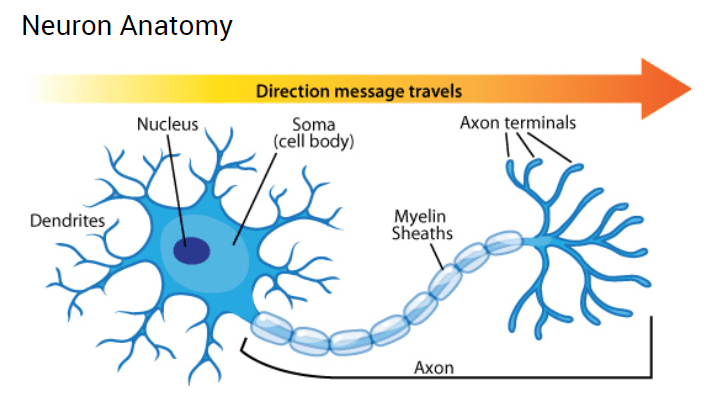
\includegraphics[scale=0.8]{chap2/c2_figs/neuron.png}
\end{center}
\caption{Cấu trúc một tế bào thần kinh}
\label{fig:neuronsinhhoc}
\end{figure}
\FloatBarrier
\centerline{Nguồn: https://askabiologist.asu.edu/neuron-anatomy}

Neuron là đơn vị cơ bản cấu tạo hệ thống thần kinh và là một phần quan trọng nhất của não. Não chúng ta gồm khoảng 10 triệu neuron và mỗi neuron liên kết với khoangr 10.000 neuron khác.

Ở mỗi neuron có phần thân (soma) chứa nhân, các tín hiệu đầu vào qua sợi nhánh (dendrites) và các tín hiệu đầu ra qua sợi trục (axon) kết nối với các neuron khác. Hiểu đơn giản mỗi neuron nhận dữ liệu đầu vào qua sợi nhánh và truyền dữ liệu đầu ra qua sợi trục, đến các sợi nhánh của các neuron khác.

Mỗi neuron nhận xung điện từ các neuron khác qua sợi nhánh. Nếu các xung điện này đủ lớn để kích hoạt neuron, thì tín hiệu này đi qua sợi trục đến các sợi nhánh của các neuron khác. => Ở mỗi neuron cần quyết định có kích hoạt neuron đấy hay không.

Tuy nhiên NN chỉ là lấy cảm hứng từ não bộ và cách nó hoạt động, chứ không phải bắt chước toàn bộ các chức năng của nó. Việc chính của chúng ta là dùng mô hình đấy đi giải quyết các bài toán chúng ta cần.

\subsection{Perceptron}
\label{s:perceptron}
\FloatBarrier
\begin{figure}[htp]
\begin{center}
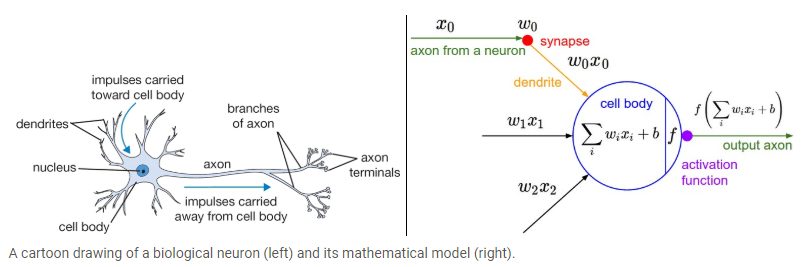
\includegraphics[scale=0.6]{chap2/c2_figs/perceptron.PNG}
\end{center}
\caption{Perceptron}
\label{fig:perceptron}
\end{figure}
\FloatBarrier

Lấy ý tưởng từ neuron sinh học, neuron nhân tạo với tên gọi perceptron cũng họat động theo cách gần giống với neuron sinh học để tạo thành một mạng thần kinh nhân tạo cho máy tính.

Đơn vị tính toán cơ bản trong một mạng NN được gọi là perceptron và thường được gọi là \textbf{node} hay \textbf{unit}. Một node nhận các đầu vào từ các nodes khác hoặc từ nguồn bên ngoài, sau đó tính toán tạo ra giá trị ngõ ra. Mỗi ngõ vào có một trọng số liên kết và giá trị này biểu thi mức độ liên quan giữa node hiện tại và node trước nó. Node áp dụng một hàm $f$ (được giới thiệu ở nội dung bên dưới) vào tổng các các tích ngõ vào và trọng số để tạo giá trị ngõ ra. Hình \ref{fig:single_neuron} miêu tả chi tiết một neuron và các hoạt động của nó.

\FloatBarrier
\begin{figure}[htp]
\begin{center}
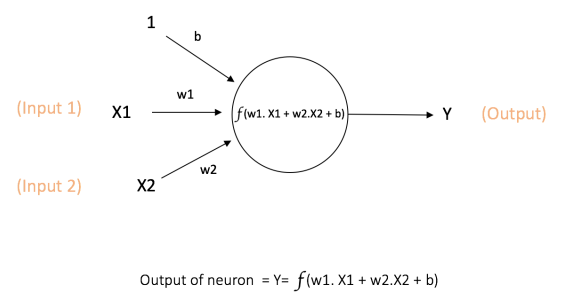
\includegraphics[scale=1]{chap2/c2_figs/single_neuron.PNG}
\end{center}
\caption{Một neuron cơ bản}
\label{fig:single_neuron}
\end{figure}
\FloatBarrier

Node trong hình \ref{fig:single_neuron} có hai đầu vào \textbf{Input 1} và \textbf{Input 2} có giá trị tương ứng $X1$ và $X2$, trọng số là \textbf{w1} và \textbf{w2}. Ngoài ra, có một đầu vào khác với giá trị \textbf{1} và trọng số b (được gọi là bias). Ngõ ra của node là Y được tính toán như hình \ref{fig:single_neuron}. Hàm \textbf{f} là hàm phi tuyến tính và được gọi là hàm kích hoạt (Activation Function). Đặc tính phi tuyến của hàm kích hoạt giúp mạng NN có thể "học" những dữ liệu thực trọng tự nhiên và hầu hết chúng đều có tính chất phi tuyến.

Các hàm kích hoạt thường được sử dụng trong thực tế:
\begin{itemize}
\item \textbf{Sigmoid:} lấy giá trị ngõ vào thực và ép nó nằm trong giới hạn [0, 1].
\begin{equation}
\sigma (x) = \frac{1}{{1 + {e^{ - x}}}}
\end{equation}
\item \textbf{Tanh:} lấy giá trị ngõ vào thực và ép nó nằm trong giới hạn [-1, 1].
\begin{equation}
\tanh (x) = 2\sigma (2x) - 1
\end{equation}
\item \textbf{ReLU:} lấy giá trị ngõ vào thực và lấy ngưỡng ở 0 (thay thế các giá trị âm bằng 0 hoặc giá trị rất nhỏ).
\begin{equation}
f(x) = \max (0,x)
\end{equation}
\end{itemize}

\noindent Đồ thị các hàm kích hoạt được mô tả trong hình \ref{fig:activation_function}.

\FloatBarrier
\begin{figure}[htp]
\begin{center}
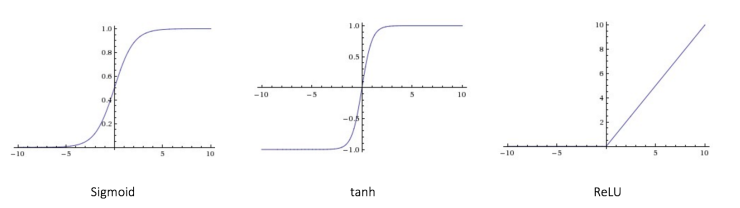
\includegraphics[scale=0.8]{chap2/c2_figs/activation_function.PNG}
\end{center}
\caption{Đồ thị các hàm kích hoạt}
\label{fig:activation_function}
\end{figure}
\FloatBarrier

Tầm quan trọng của bias: 

\subsection{Kiến trúc mạng Neuron Network}

Một mạng NN được xây dựng gồm nhiều lớp (layer). Mỗi lớp được cấu thành từ nhiều node cơ bản (đã trình bày trong mục \ref{s:perceptron}). Ngõ ra của các node ở lớp phía trước là ngõ vào của các node lớp phía sau, chúng được gọi là các liên kết (connection) và tương ứng với các trọng số khác nhau.

\FloatBarrier
\begin{figure}[htp]
\begin{center}
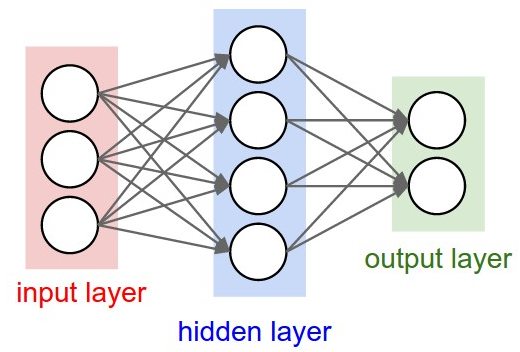
\includegraphics[scale=0.8]{chap2/c2_figs/structure_NN.PNG}
\end{center}
\caption{Mạng Neural Network cơ bản}
\label{fig:structure_NN}
\end{figure}
\FloatBarrier

Một mạng NN cơ bản sẽ có 3 tầng (minh họa trong hình \ref{fig:structure_NN}):
\begin{itemize}
\item \textbf{Tầng vào} (\textit{input layer}): Là tầng bên trái cùng của mạng thể hiện cho các đầu vào của mạng.
\item \textbf{Tầng ra} (\textit{output layer}): Là tầng bên phải cùng của mạng thể hiện cho các đầu ra của mạng.
\item \textbf{Tầng ẩn} (\textit{hidden layer}): Là tầng nằm giữa tầng vào và tầng ra thể hiện cho việc suy luận logic của mạng.
\end{itemize}

Một mạng NN chỉ có một tầng vào và một tầng ra, nhưng có thể có nhiều tầng ẩn. Số lượng tầng ẩn phụ thuộc vào độ phức tạp của bài toán được mạng NN giải quyết và được thiết kế dựa trên kinh nghiệm của người xây dựng mạng.

\subsection{Hoạt động của mạng}
\label{hoat_dong_cua_mang}

Tín hiệu đầu vào (gồm các thông tin cần dự đoán) sẽ được truyền từ input layer. Sau đó được tính toán qua các hidden layer bới các nodes. Cuối cùng output layer sẽ thực hiện việc dự đoán và phân lọai.\\

Mỗi node trong hidden layer và output layer sẽ thực hiện các công việc sau:
\begin{itemize}
\item Liên kết với tất cả các node ở layer trước đó với các hệ số $w$ riêng.
\item Mỗi node có 1 hệ số bias b riêng.
\item Diễn ra 2 bước: tính tổng linear và áp dụng activation function đưa ra output của node.
\end{itemize}

Để hiểu rõ ràng nhất, ta đi sâu vào các tính toán trong một mạng NN cụ thể như hình \ref{fig:NN}.\\

\FloatBarrier
\begin{figure}[htp]
\begin{center}
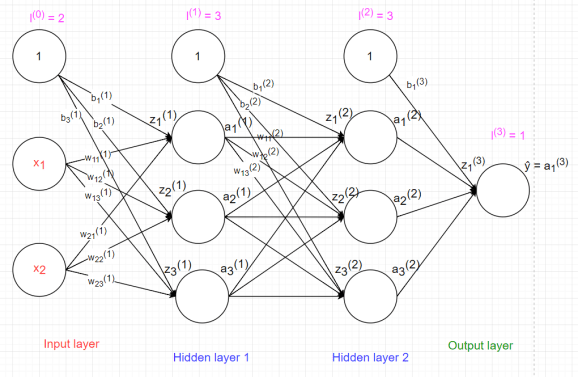
\includegraphics[scale=1]{chap2/c2_figs/nn_full-2.png}
\end{center}
\caption{Mô hình neural network trên gồm 3 layer. Input layer có 2 node $(l^{(0)} = 2$, hidden layer 1 có 3 node, hidden layer 2 có 3 node và output layer có 1 node.}
\label{fig:NN}
\end{figure}
\FloatBarrier

\textbf{Ký hiệu:}
\begin{itemize}
\item Số node trong hidden layer thứ $i$ là $l^{(i)}l(i)$.

\item Ma trận $W^{(k)}$ kích thước $l^{(k-1)}*l^{(k)}$ là ma trận hệ số giữa layer $(k-1)$ và layer $k$, trong đó $w_{ij}^{(k)}$ là hệ số kết nối từ node thứ $i$ của layer $k-1$ đến node thứ $j$ của layer $k$.

\item Vector $b^{(k)}$ kích thước $l^{k} * 1$ là hệ số bias của các node trong layer $k$, trong đó $b_i^{(k)}$ là bias của node thứ $i$ trong layer $k$. 
\end{itemize}

Với node thứ $i$ trong layer $l$ có bias $b_i^{(l)}$ thực hiện 2 bước:
\begin{itemize}
\item Tính tổng linear: $z_i^{(l)} = \sum_{j=1}^{l^{(l-1)}} a_j^{(l-1)} * w_{ji}^{(l)} + b_i^{(l)}$ là tổng tất cả các node trong layer trước nhân với hệ số w tương ứng, rồi cộng với bias b.
\item Áp dụng activation function: $a_i^{(l)} = \sigma(z_i^{(l)})$
\end{itemize}

Vector $z^{(k)}$ kích thước $l^{(k)} * 1$ là giá trị các node trong layer $k$ sau bước tính tổng linear.

Vector $a^{(k)}$ kích thước $l^{(k)} * 1$ là giá trị của các node trong layer $k$ sau khi áp dụng hàm activation function.



Do mỗi node trong hidden layer và output layer đều có bias nên trong input layer và hidden layer cần thêm node 1 để tính bias (nhưng không tính vào tổng số node layer có).

Tại node thứ 2 ở layer 1, ta có:

\begin{itemize}
\item $z_2^{(1)} =  x_1 * w_{12}^{(1)} +  x_2 * w_{22}^{(1)} + b_2^{(1)}$
\item $a_2^{(1)} = \sigma(z_2^{(1)})$
\end{itemize} 

Hay ở node thứ 3 layer 2, ta có:
\begin{itemize}
\item $z_3^{(2)} =  a_1^{(1)} * w_{13}^{(2)} + a_2^{(1)} * w_{23}^{(2)}  + a_3^{(1)} * w_{33}^{(2)} + b_3^{(2)}$
\item $a_2^{(1)} = \sigma(z_2^{(1)})$
\end{itemize} 

\subsection{Quá trình huấn luyện một mạng NN}

Quá trình huấn luyện một mạng NN được thể hiện qua sự lặp đi lặp lại hai bước sau:
\begin{itemize}
\item \textbf{Feedforward:} Lan truyền tiến. Dự đoán output $\hat{y}$ với một input $x$ bằng cách tính toán từ đầu đến cuối của mạng neuron.
\item \textbf{Backpropagation:} Lan truyền ngược và cập nhật trọng số.
\end{itemize}
\textbf{Bước 1: Lan truyền tiến}
Để nhất quán về mặt ký hiệu, gọi input layer là $a^{(0)} (=x)$ kích thước $2*1$.


\FloatBarrier
\begin{figure}[htp]
\begin{center}
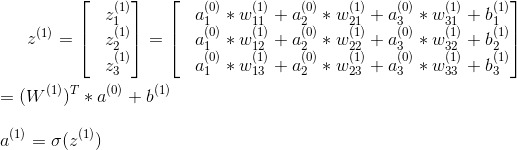
\includegraphics[scale=0.8]{chap2/c2_figs/feed_forward.jpg}
\end{center}
\label{fig:feed_forward0}
\end{figure}
\FloatBarrier
Tương tự ta có:
$\newline z^{(2)} = (W^{(2)})^T * a^{(1)} + b^{(2)}\newline  a^{(2)} = \sigma(z^{(2)}) \newline z^{(3)} = (W^{(3)})^T * a^{(2)} + b^{(3)}\newline  \hat{y} = a^{(3)} = \sigma(z^{(3)})$

\FloatBarrier
\begin{figure}[htp]
\begin{center}
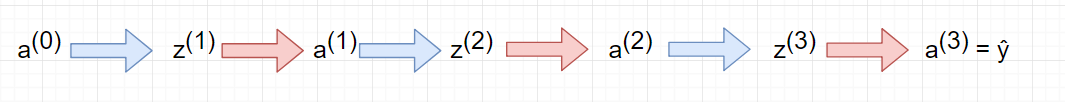
\includegraphics[scale=0.75]{chap2/c2_figs/ff.png}
\end{center}
\caption{Feedforward}
\label{fig:feed_forward}
\end{figure}
\FloatBarrier

\begin{itemize}
\item[$\square$] \textbf{Biểu diễn dưới dạng ma trận:}
\end{itemize}
Tuy nhiên khi làm việc với dữ liệu ta cần tính dự đoán cho nhiều dữ liệu một lúc, nên gọi $X$ là ma trận $n*d$, trong đó $n$ là số dữ liệu và $d$ là số trường trong mỗi dữ liệu, trong đó $x_j^{[i]}$ là giá trị trường dữ liệu thứ $j$ của dữ liệu thứ $i$.
Biểu diễn dạng ma trận của vector dữ liệu đầu vào như sau:

\FloatBarrier
\begin{figure}[htp]
\begin{center}
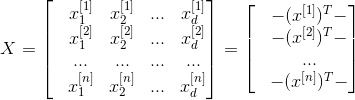
\includegraphics[scale=0.8]{chap2/c2_figs/1.jpg}
\end{center}
\label{fig:feed_forward}
\end{figure}
\FloatBarrier

Do $x^{[1]}$ là vector kích thước $d*1$ tuy nhiên ở $X$ mỗi dữ liệu được viết theo hàng nên cần transpose $x^{[1]}$ thành kích thước $1*d$, kí hiệu: $(x^{[1]})^T$
Gọi ma trận $Z^{(i)}$ kích thước$ N*l^{(i)}$ trong đó $z_{j}^{(i)[k]}$ là giá trị thứ $j$ trong layer $i$ sau bước tính tổng linear của dữ liệu thứ $k$ trong dataset.

*** Kí hiệu $(i)$ là layer thứ $i$ và kí hiệu $[k]$ là dữ liệu thứ $k$ trong dataset.

Tương tự, gọi ma trận $A^{(i)}$ kích thước $N*l^{(i)}$ trong đó $a_{j}^{(i)[k]}$ là giá trị thứ $j$ trong layer $i$ sau khi áp dụng activation function của dữ liệu thứ $k$ trong dataset.

\FloatBarrier
\begin{figure}[htp]
\begin{center}
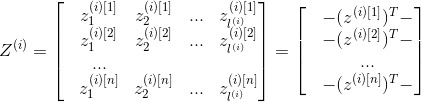
\includegraphics[scale=0.8]{chap2/c2_figs/2.jpg}
\end{center}
\label{fig:feed_forward}
\end{figure}
\FloatBarrier

Do đó:

\FloatBarrier
\begin{figure}[htp]
\begin{center}
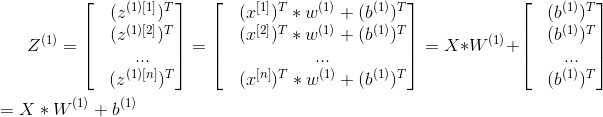
\includegraphics[scale=0.75]{chap2/c2_figs/3.jpg}
\end{center}
\label{fig:feed_forward}
\end{figure}
\FloatBarrier
Như vậy:

\FloatBarrier
\begin{figure}[htp]
\begin{center}
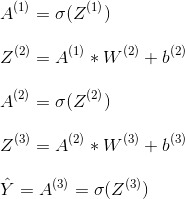
\includegraphics[scale=0.75]{chap2/c2_figs/4.jpg}
\end{center}
\label{fig:feed_forward}
\end{figure}
\FloatBarrier

Vậy là có thể tính được giá trị dự đoán của nhiều dữ liệu 1 lúc dưới dạng ma trận.

Giờ từ input $X$ ta có thể tính được giá trị dự đoán $\hat{Y}$, tuy nhiên việc chính cần làm là đi tìm hệ số $W$ và $b$. Có thể nghĩ ngay tới thuật toán gradient descent và việc quan trọng nhất trong thuật toán gradient descent là đi tìm đạo hàm của các hệ số đối với loss function. Và việc tính đạo hàm của các hệ số trong neural network được thực hiện bởi thuật toán backpropagation, sẽ được trình bày ở bước sau.

\textbf{Bước 2: Backpropagation - Lan truyền ngược và cập nhật trọng số}
Giờ ta cần đi tìm hệ số $W$ và $b$. Có thể nghĩ ngay tới thuật toán gradient descent và việc quan trọng nhất trong thuật toán gradient descent là đi tìm đạo hàm của các hệ số đối với loss function. Bước này sẽ tính đạo hàm của các hệ số trong neural network với thuật toán backpropagation.

Quá trình học vẫn là tìm lấy một hàm lỗi để đánh giá và tìm cách tối ưu hàm lỗi đó để được kết quả hợp lý nhất có thể. Với mỗi điểm $(x^{[i]}, y_i)$ ta có hàm loss function được tính theo công thức: $$L = -(y_i * log(\hat{y_i}) + (1 - y_i) * log(1 - \hat{y_i}))$$

Hàm loss function trên toàn bộ dữ liệu:
$$J = - \sum_{i=1}^{N}(y_i * log(\hat{y_i}) + (1 - y_i) * log(1 - \hat{y_i}))$$

\begin{itemize}
\item[$\blacksquare$] \textbf{Gradient Descent}
\end{itemize}
Để áp dụng gradient descent ta cần tính được đạo hàm của các hệ số W và bias b với hàm loss function.
*** Kí hiệu chuẩn về đạo hàm
\begin{itemize}
\item Khi hàm f(x) là hàm 1 biến x, ví dụ: $ f(x) = 2*x + 1$. Đạo hàm của $f$ đối với biến $x$ kí hiệu là $\frac{df}{dx}\newline $
\item Khi hàm $f(x, y)$ là hàm nhiều biến, ví dụ $ f(x, y) = x^2 + y^2$. Đạo hàm $f$ với biến $x$ kí hiệu là $ \frac{\partial f}{\partial x}$
\end{itemize}

Với mỗi điểm $(x^{([i]}, y_i)$, hàm loss function sẽ là:

$$L = -(y_i * log(\hat{y_i}) + (1 - y_i) * log(1 - \hat{y_i}))$$


trong đó: $\hat{y_i} = a_1^{(2)} = \sigma(a_1^{(1)} * w_{11}^{(2)} + a_2^{(1)} * w_{21}^{(2)} + b_1^{(2)})$
 là giá trị mà model dự đoán, còn $y_i$ là giá trị thật của dữ liệu.
$$\frac{\partial L}{\partial\hat{y_i}} = - \frac{\partial(y_i * log(\hat{y_i}) + (1 - y_i) * log(1 - \hat{y_i}))}{\partial\hat{y_i}}= - (\frac{y_i}{\hat{y_i}} - \frac{1-y_i}{(1-\hat{y})})\newline$$
Tính đạo hàm L với $W^{(2)}$, $b^{(2)}$\\
Áp dụng chain rule ta có: $$ \frac{\partial L}{\partial b_1^{(2)}} = \frac{dL}{d\hat{y_i}} * \frac{\partial\hat{y_i}}{\partial b_1^{(2)} } $$

\FloatBarrier
\begin{figure}[htp]
\begin{center}
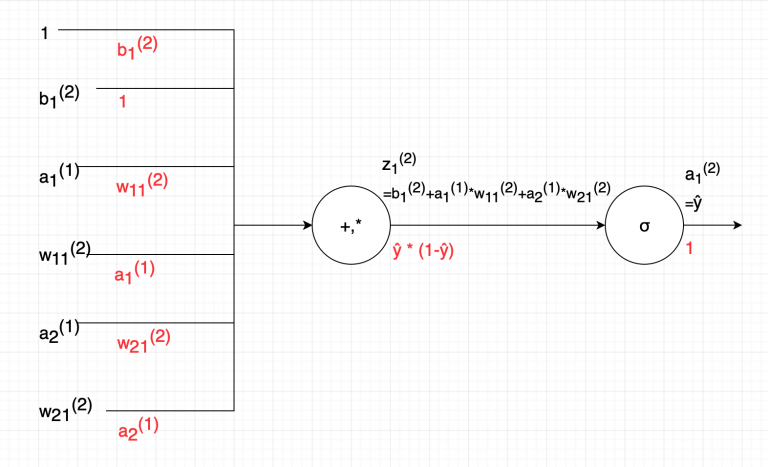
\includegraphics[scale=1]{chap2/c2_figs/6.png}
\end{center}
\label{fig:feed_forward}
\end{figure}
\FloatBarrier

Từ đồ thị ta thấy:

$$\frac{\partial\hat{y_i}}{\partial b_1^{(2)}} = \hat{y_i} * (1-\hat{y_i})\newline$$

$$\frac{\partial\hat{y_i}}{\partial w_{11}^{(2)}} = a_1^{(1)}*\hat{y_i} * (1-\hat{y_i})\newline$$

$$\frac{\partial\hat{y_i}}{\partial w_{21}^{(2)}} = a_2^{(1)}*\hat{y_i} * (1-\hat{y_i})\newline$$

$$\frac{\partial\hat{y_i}}{\partial a_1^{(1)} }=w_{11} ^{(2)}*\hat{y_i} * (1-\hat{y_i})\newline$$

$$\frac{\partial\hat{y_i}}{\partial a_2^{(1)} }=w_{21} ^{(2)}*\hat{y_i} * (1-\hat{y_i})\newline$$
Do đó:
$$\frac{\partial L}{\partial b_1^{(2)}} = \frac{\partial L}{\partial\hat{y_i}} * \frac {\partial\hat{y_i}}{\partial b_1^{(2)}} = - (\frac{y_i}{\hat{y_i}} - \frac{1-y_i}{(1-\hat{y_i})}) * \hat{y_i} * (1-\hat{y_i}) = -(y_i * (1-\hat{y_i}) - (1-y_i) * \hat{y_i})) = \hat{y_i}-y_i$$

Tương tự:
$$\frac{\partial L}{\partial w_{11} ^ {(2)}} = a_1 ^ {(1)} *     (\hat{y_i}-y_i)\newline \newline$$

$$\frac{\partial L}{\partial w_{21} ^ {(2)}} = a_2 ^ {(1)} *     (\hat{y_i}-y_i) \newline \newline$$

$$\frac{\partial L}{\partial a_1 ^ {(1)}} =  w_{11} ^ {(2)}  *     (\hat{y_i}-y_i) \newline \newline$$

$$\frac{\partial L}{\partial a_2 ^ {(1)}} =  w_{21} ^ {(2)}  *     (\hat{y_i}-y_i) \newline \newline $$


\begin{itemize}
\item[$\square$] \textbf{Biểu diễn dưới dạng ma trận:}
\end{itemize} 
\textbf{*** Lưu ý:} đạo hàm của L đối với ma trận W kích thước m*n cũng là một ma trận cùng kích thước $m*n$.

\FloatBarrier
\begin{figure}[htp]
\begin{center}
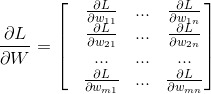
\includegraphics[scale=1]{chap2/c2_figs/5.jpg}
\end{center}
\label{fig:feed_forward}
\end{figure}
\FloatBarrier

Do đó:
$$\frac{\partial J}{\partial W^{(2)}} = (A^{(1)})^T * (\hat{Y} - Y), \frac{\partial J}{\partial b^{(2)}} = (sum(\hat{Y} - Y))^T,  \frac{\partial J}{\partial A^{(1)}} = (\hat{Y} - Y) * (W^{(2)})^T$$ 
là phép tính sum tính tổng các cột của ma trận.

\FloatBarrier
\begin{figure}[htp]
\begin{center}
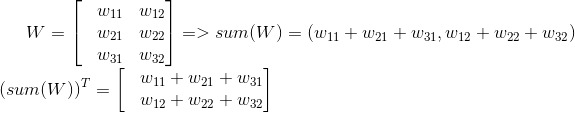
\includegraphics[scale=0.8]{chap2/c2_figs/6.jpg}
\end{center}
\label{fig:feed_forward}
\end{figure}
\FloatBarrier

Vậy là đã tính xong đạo hàm của $L$ với hệ số $W^{(2)}, b^{(2)}$. Giờ sẽ đi tính đạo hàm của $L$ với hệ số $W^{(1)}, b^{(1)}$ để khi tính đạo hàm của hệ số và bias trong layer trước đấy sẽ cần dùng đến.

Tính đạo hàm L với $W^{(1)}, b^{(1)}$
Do $ a_1^{(1)} = \sigma(b_1^{(1)} + x_1*w_{11}^{(1)} + x_2*w_{21}^{(1)})$ 

Áp dụng chain rule ta có: $$ \frac{\partial L}{\partial b_1^{(1)}} = \frac{\partial L}{\partial a_1^{(1)}} * \frac{\partial a_1^{(1)}}{\partial b_1^{(1)} }$$
Ta có:
$$\frac{\partial a_1^{(1)}}{\partial b_1^{(1)}} = \frac{\partial a_1^{(1)}}{z_1^{(1)}} * \frac{z_1^{(1)}}{\partial b_1^{(1)}} = a_1^{(1)} * (1 - a_1^{(1)})$$
Do đó:
$$\frac{\partial L}{\partial b_1^{(1)}} = a_1 ^ {(1)} * (1 - a_1^{(1)}) * w_{11}^{(2)} * (\hat{y_i} - y_i)$$

Tương tự:
$$\frac{\partial L}{\partial w_{11}^{(1)}} = x_1 * a_1 ^ {(1)} * (1 - a_1^{(1)}) * w_{11}^{(2)} *  (\hat{y_i} - y_i)  \newline$$

$$\frac{\partial L}{\partial w_{12}^{(1)}} = x_1 * a_2 ^ {(1)} * (1 - a_2^{(1)}) * w_{11}^{(2)} *  (\hat{y_i} - y_i)  \newline$$

$$\frac{\partial L}{\partial w_{21}^{(1)}} = x_2 * a_1 ^ {(1)} * (1 - a_1^{(1)}) * w_{21}^{(2)} *  (\hat{y_i} - y_i)  \newline $$

$$\frac{\partial L}{\partial w_{22}^{(1)}} = x_2 * a_2^ {(1)} * (1 - a_2^{(1)}) * w_{21}^{(2)} *  (\hat{y_i} - y_i)  \newline$$

Có thể tạm viết dưới dạng chain rule là: $$\frac{\partial J}{\partial W^{(1)}} = \frac{\partial J}{\partial A^{(1)}} * \frac{\partial A^{(1)}}{\partial Z^{(1)}}* \frac{\partial Z^{(1)}}{\partial W^{(1)}} (1) $$

Từ trên đã tính được: $$\frac{\partial J}{\partial A^{(1)}} = (\hat{Y} - Y) * (W^{(2)})^T$$

Đạo hàm của hàm sigmoid: $\frac{d\sigma(x)}{dx} = \sigma(x) * (1 - \sigma(x))$ và $A^{(1)} = \sigma(Z^{(1)})$ , nên trong (1) có thể hiểu là $\frac{\partial A^{(1)}}{\partial Z^{(1)}} = A^{(1)}* (1 - A^{(1)})$

Cuối cùng, $Z^{(1)} = X * W^{(1)} + b^{(1)}$ nên có thể tạm hiểu $\frac{\partial Z^{(1)}}{\partial W^{(1)}} = X$ , nó giống như $f(x)= a*x +b$ $ => \frac{df}{dx} = a$ .

Kết hợp tất cả lại ta được:
$$\frac{\partial J}{\partial W^{(1)}} = X^T * (((\hat{Y} – Y) * (W^{(2)})^T)\otimes A^{(1)}\otimes (1-A^{(1)}) ) $$

Vậy khi nào cần dùng element-wise $(\otimes)$, khi nào dùng nhân ma trận $(*)$?
\begin{itemize}
\item Khi tính đạo hàm ngược lại qua bước activation thì dùng $(\otimes)$.
\item Khi có phép tính nhân ma trận thì dùng $(*)$, nhưng đặc biệt chú ý đến \textbf{kích thước ma trận} và dùng \textbf{transpose} nếu cần thiết. Ví dụ: ma trận $X$ kích thước $N*3$, W kích thước $3*4$, $Z = X * W$ sẽ có kích thước $N*4$ thì $\frac{\partial J}{\partial W} = X^T * (\frac{\partial J}{\partial Z})$ và $\frac{\partial J}{\partial X} = (\frac{\partial J}{\partial Z}) * W^T$.
\end{itemize}
Tương tự: $$\frac{\partial L}{\partial b^{(1)}} = sum(((\hat{Y} – Y) * (W^{(2)})^T)\otimes A^{(1)})^T$$

Vậy là đã tính xong hết đạo hàm của loss function với các hệ số $W$ và bias $b$, giờ có thể áp dụng gradient descent để giải bài toán.

Giờ thử tính $ \frac{\partial L}{\partial x_1}$, ở bài này thì không cần vì chỉ có 1 hidden layer, nhưng nếu nhiều hơn 1 hidden layer thì cần phải tính bước này để tính đạo hàm với các hệ số trước đó.

\FloatBarrier
\begin{figure}[htp]
\begin{center}
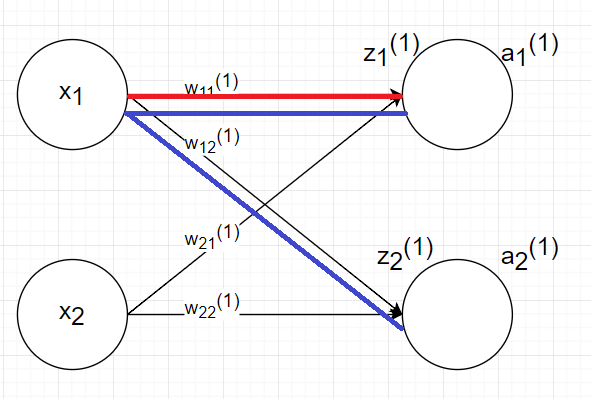
\includegraphics[scale=0.75]{chap2/c2_figs/1.png}
\end{center}
\caption{Đường màu đỏ cho $w_{11}^{(1)}$, đường màu xanh cho $x_1$}
\label{fig:feed_forward}
\end{figure}
\FloatBarrier

Ta thấy $w_{11}^{(1)}$ chỉ tác động đến $a_1^{(1)}$, cụ thể là $ a_1^{(1)} = \sigma(b_1^{(1)} + x_1*w_{11}^{(1)} + x_2*w_{21}^{(1)})$ 

Tuy nhiên $x_1$ không những tác động đến $a_1^{(1)}$ mà còn tác động đến $a_2^{(1)}$, nên khi áp dụng chain rule tính đạo hàm của $L$ với $x_1$ cần tính tổng đạo hàm qua cả $a_1^{(1)}$ và $a_2^{(1)}$.

\FloatBarrier
\begin{figure}[htp]
\begin{center}
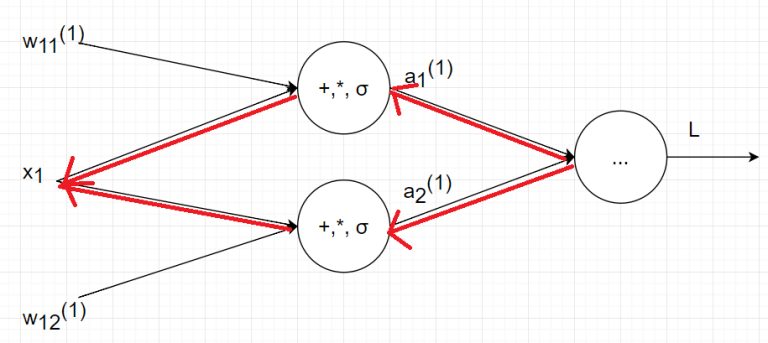
\includegraphics[scale=0.75]{chap2/c2_figs/2.png}
\end{center}
\caption{backpropagation tác động trong lớp ẩn}
\label{fig:feed_forward}
\end{figure}
\FloatBarrier

Do đó:
$$\frac{\partial L}{\partial x_1} = \frac{\partial L}{\partial a_1^{(1)}} * \frac{\partial a_1^{(1)}}{\partial x_1} + \frac{\partial L}{\partial a_2^{(1)}} * \frac{\partial a_2^{(1)}}{\partial x_1} =  w_{11}^{(1)}* a_1 ^ {(1)} * (1 – a_1^{(1)}) * w_{11}^{(2)} * (y_i – \hat{y_i}) + w_{12}^{(1)}* a_2 ^ {(1)} * (1 – a_2^{(1)}) * w_{21}^{(2)} * (y_i – \hat{y_i})  \newline$$

Sau tất cả, mô hình tổng quát sẽ bao gồm các bước như sau:

\FloatBarrier
\begin{figure}[htp]
\begin{center}
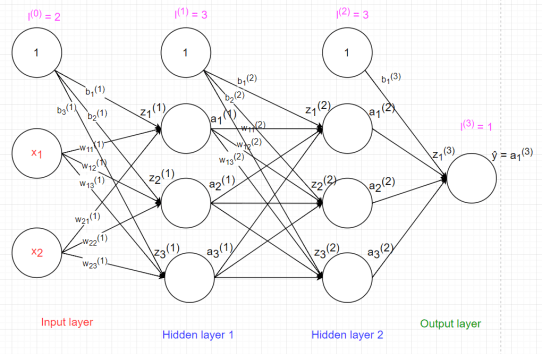
\includegraphics[scale=0.75]{chap2/c2_figs/3.png}
\end{center}
\caption{Mô hình neural network}
\label{fig:feed_forward}
\end{figure}
\FloatBarrier

\begin{itemize}
\item \textbf{Bước 1:} Tính $\frac{\partial J}{\partial \hat{Y}}$, trong đó $\hat{Y} = A^{(3)}$
\item \textbf{Bước 2:} Tính $$\frac{\partial J}{\partial \hat{W^{(3)}}}= (A^{(2)})^T * (\frac{\partial J}{\partial \hat{Y}} \otimes \frac{\partial A^{(3)}}{\partial Z^{(3)}}),  \frac{\partial J}{\partial \hat{b^{(3)}}}= (sum( \frac{\partial J}{\partial \hat{Y}} \otimes \frac{\partial A^{(3)}}{\partial Z^{(3)}}))^T$$
\item \textbf{Bước 3:} Tính $$\frac{\partial J}{\partial \hat{W^{(2)}}}= (A^{(1)})^T * (\frac{\partial J}{\partial A^{(2)}} \otimes \frac{\partial A^{(2)}}{\partial Z^{(2)}}),  \frac{\partial J}{\partial \hat{b^{(2)}}}= (sum (\frac{\partial J}{\partial A^{(2)}} \otimes \frac{\partial A^{(2)}}{\partial Z^{(2)}}))^T$$ và tính $$\frac{\partial J}{\partial \hat{A^{(1)}}}= ( \frac {\partial J}{\partial A^{(2)}} \otimes \frac{\partial A^{(2)}}{\partial Z^{(2)}}) * (W^{(2)})^T$$ 
\item \textbf{Bước 4:} Tính $$\frac{\partial J}{\partial \hat{W^{(1)}}}= (A^{(0)})^T  * (\frac{\partial J}{\partial A^{(1)}} \otimes \frac{\partial A^{(1)}}{\partial Z^{(1)}}),  \frac{\partial J}{\partial \hat{b^{(1)}}}= (sum (\frac{\partial J}{\partial A^{(1)}} \otimes \frac{\partial A^{(1)}}{\partial Z^{(1)}}))^T$$ , trong đó $A^{(0)} = X$
\end{itemize}

Nếu network có nhiều layer hơn thì cứ tiếp tục cho đến khi tính được đạo hàm của loss function $J$ với tất cả các hệ số $W$ và bias $b$.

Nếu hàm activation là sigmoid thì $\frac{\partial A^{(i)}}{\partial Z^{(i)}} = A^{(i)} \otimes (1-A^{(i)})$

Tổng kết lại, 2 quá trình Feedfoward và Backpropagation sẽ diễn ra lần lượt như sau:

\FloatBarrier
\begin{figure}[htp]
\begin{center}
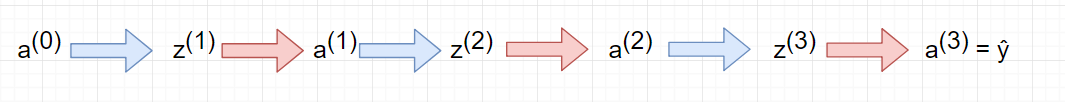
\includegraphics[scale=0.7]{chap2/c2_figs/7.png}
\end{center}
\end{figure}
\FloatBarrier

\FloatBarrier
\begin{figure}[htp]
\begin{center}
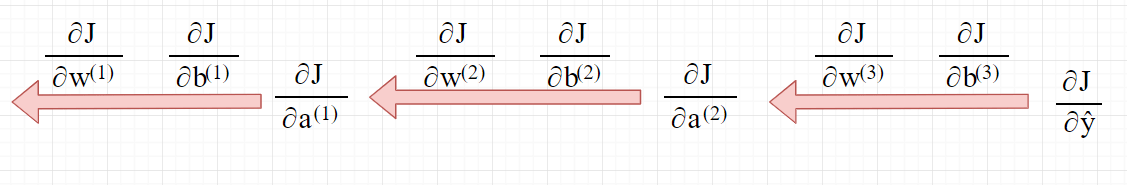
\includegraphics[scale=0.65]{chap2/c2_figs/8.png}
\end{center}
\caption{Feedforward và Backpropagation}
\label{fig:backpropagation}
\end{figure}
\FloatBarrier

(Theo "Sách Deep Learning cơ bản" - tác giả: Nguyễn Thanh Tuấn)

\section{Mạng Convolutional Neural Network (CNN)}
Convolutional Neural Network (CNNs – Mạng nơ-ron tích chập) là một trong những mô hình Deep Learning tiên tiến giúp cho chúng ta xây dựng được những hệ thống thông minh với độ chính xác cao như hiện nay. Trong luận văn này, sẽ trình bày về Convolution (tích chập) đi từ những khái niệm cơ bản nhất đến ứng dụng của nó cũng như ý tưởng của mô hình CNNs trong phát hiện và trích xuất đặc trưng khung xương từ ảnh RGB.

Mạng Neural Network truyền thống tuy đã giải quyết  được một số vấn đề lớn lúc bấy giờ nhưng lại gặp một số khó khăn khi giải quyết bài toán xử lý, phân loại hình ảnh.
Đối với mạng Neural Network truyền thống khi xử lý ảnh màu 64*64 được biểu diễn dưới dạng 1 tensor 64*64*3. Việc để biểu thị hết nội dung của bức ảnh thì cần truyền vào input layer tất cả các pixel (64*64*3 = 12288). Nghĩa là input layer giờ có 12288 nodes. Giả sử số lượng node trong hidden layer 1 là 1000. Số lượng weight $W$ giữa input layer và hidden layer 1 là 12288*1000 = 12288000, số lượng bias là 1000 $=>$ tổng số parameter là: 12289000. Đây mới chỉ là số parameter giữa input layer và hidden layer 1, trong model còn nhiều layer nữa, và nếu kích thướcây ảnh tăng, ví dụ 512*512 thì số lượng parameter tăng cực kì nhanh. Điều này khiến cho việc tính toán của máy tính cần rất nhiều công sức nhưng lại không mang lại hiệu quả cao. Do vậy ta cần có giải pháp tốt hơn.

Nhận xét:
\begin{itemize}
\item Trong ảnh các pixel ở cạnh nhau thường có liên kết với nhau hơn là những pixel ở xa. Ví dụ để thể hiện một vật thể trên ảnh cần các pixel gần nhau và có màu sắc tương tự nhau.
\item Ngoài ra để so sánh các đối tượng là giống hay khác nhau cần phải so sánh giữa khu vực này với khu vực kia của bức ảnh. Do vậy cần phải có một bộ hệ số tính toán với các pixel quét hết toàn bộ bức ảnh để so sánh các vùng. Hay nói cách khác là các pixel ảnh chia sẻ hệ số với nhau.
\end{itemize}
=> Do vậy ý tưởng sử dụng mạng Convolutional Neural Network ra đời. Áp dụng phép tính convolution vào layer trong neural network ta có thể giải quyết được vấn đề lượng lớn parameter mà vẫn lấy ra được các đặc trưng của ảnh.
\subsection{Phép Tính Convolution}
\label{ss: convolution}
Để cho dễ hình dung mình sẽ lấy ví dụ trên ảnh xám, tức là ảnh được biểu diễn dưới dạng ma trận $A$ kích thước $m*n$.
Ta định nghĩa kernel là một ma trận vuông kích thước $k*k$ trong đó $k$ là số lẻ. $k$ có thể bằng $1, 3, 5, 7, 9,…$ Ví dụ kernel kích thước $3*3$.

Kí hiệu phép tính convolution $(\otimes)$, kí hiệu $Y = X \otimes W$.

Với mỗi phần tử $x_{ij}$ trong ma trận $X$ lấy ra một ma trận có kích thước bằng kích thước của kernel $W$ có phần tử $x_{ij}$ làm trung tâm (đây là vì sao kích thước của kernel thường lẻ) gọi là ma trận $A$. Sau đó tính tổng các phần tử của phép tính element-wise của ma trận $A$ và ma trận $W$, rồi viết vào ma trận kết quả $Y$.

\FloatBarrier
\begin{figure}[htp]
\begin{center}
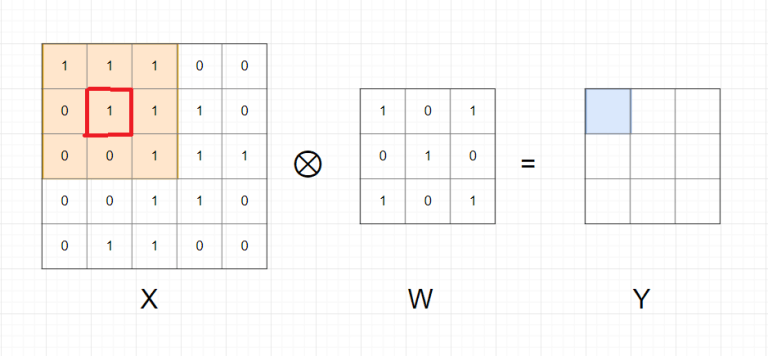
\includegraphics[scale=0.65]{chap2/c2_figs/9.png}
\end{center}
\caption{Phép tính Convolution}
\label{fig:convolution}
\end{figure}
\FloatBarrier

Ví dụ khi tính tại $x_{22}$ (ô khoanh đỏ trong hình \ref{fig:convolution}), ma trận $A$ cùng kích thước với $W$, có $x_{22}$ làm trung tâm có màu nền da cam như trong hình. Sau đó tính $y_{11} = sum(A \otimes W) = x_{11}*w_{11} + x_{12}*w_{12} + x_{13}*w_{13} + x_{21}*w_{21} + x_{22}*w_{22} + x_{23}*w_{23} + x_{31}*w_{31} + x_{32}*w_{32} + x_{33}*w_{33} = 4$. Và làm tương tự với các phần tử còn lại trong ma trận.

Vì tâm của kernel $W$ không thể lướt hết ma trận $X$ nên $Y$ sẽ có kích thước nhỏ hơn ma trận $X$. Kích thước của ma trận Y là (m-k+1) * (n-k+1).

\FloatBarrier
\begin{figure}[htp]
\begin{center}
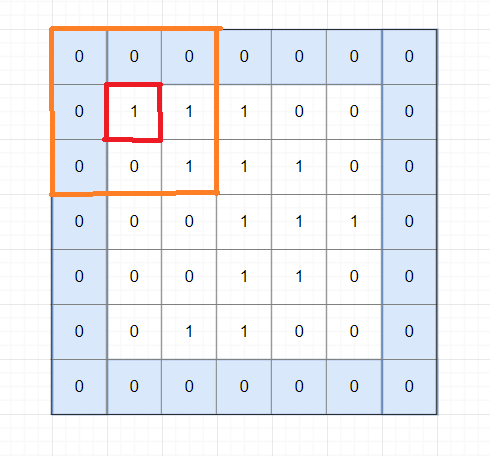
\includegraphics[scale=0.65]{chap2/c2_figs/10.png}
\end{center}
\caption{Convolution feature có kích thước nhỏ hơn ảnh ban đầu}
\label{fig:convolution-feature}
\end{figure}
\FloatBarrier

\begin{itemize}
\item[$\blacksquare$] \textbf{Padding}
Mỗi lần thực hiện phép tính convolution xong thì kích thước ma trận Y đều nhỏ hơn X. Tuy nhiên giờ ta muốn ma trận Y thu được có kích thước bằng ma trận X vì vậy cần tìm cách giải quyết cho các phần tử ở viền bằng cách thêm giá trị 0 ở viền ngoài ma trận X.

\FloatBarrier
\begin{figure}[htp]
\begin{center}
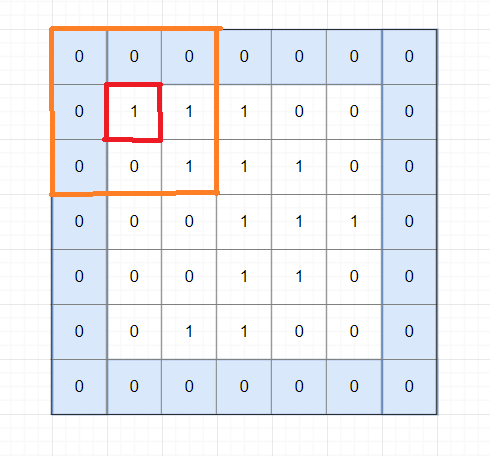
\includegraphics[scale=0.65]{chap2/c2_figs/10.png}
\end{center}
\caption{Ma trận X có viền 0 bên ngoài}
\label{fig:padding}
\end{figure}
\FloatBarrier

Rõ ràng là giờ đã giải quyết được vấn đề tìm A cho phần tử $x_{11}$, và ma trận $Y$ thu được sẽ bằng kích thước ma trận $X$ ban đầu.

Phép tính này gọi là convolution với $padding=1$. $Padding=k$ nghĩa là thêm $k$ vector $0$ vào mỗi phía của ma trận.

\item[$\blacksquare$] \textbf{Stride}
Như ở trên ta thực hiện tuần tự các phần tử trong ma trận $X$, thu được ma trận $Y$ cùng kích thước ma trận $X$, ta gọi là $stride=1$.

\FloatBarrier
\begin{figure}[htp]
\begin{center}
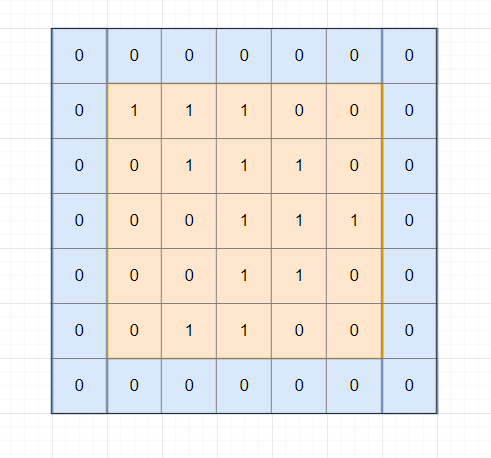
\includegraphics[scale=0.65]{chap2/c2_figs/11.png}
\end{center}
\caption{$stride=1, padding=1$}
\label{fig:padding}
\end{figure}
\FloatBarrier

Tuy nhiên nếu $stride=k (k > 1)$ thì ta chỉ thực hiện phép tính convolution trên các phần tử $x_{1+i*k,1+j*k}$. Ví dụ $k = 2$.

\FloatBarrier
\begin{figure}[htp]
\begin{center}
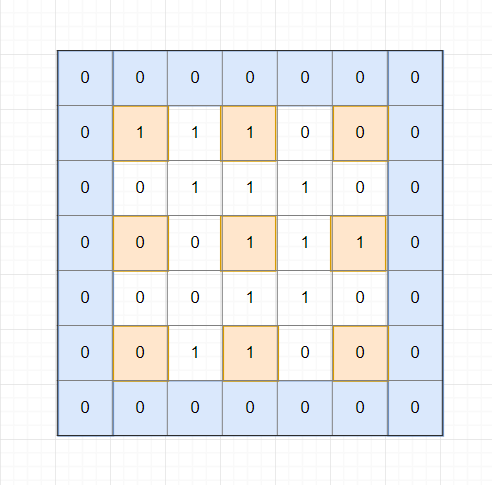
\includegraphics[scale=0.65]{chap2/c2_figs/12.png}
\end{center}
\caption{$padding=1, stride=2$}
\label{fig:padding,stride}
\end{figure}
\FloatBarrier

Hiểu đơn giản là bắt đầu từ vị trí $x_{11}$ sau đó nhảy $k$ bước theo chiều dọc và ngang cho đến hết ma trận $X$.

Kích thước của ma trận $Y$ là $3*3$ đã giảm đi đáng kể so với ma trận $X$.
Công thức tổng quát cho phép tính convolution của ma trận $X$ kích thước $m*n$ với kernel kích thước $k*k$, $stride = s$, $padding = p$ ra ma trận $Y$ kích thước $$(\frac{m-k+2p}{s}+1) * (\frac{n-k+2p}{s}+1)$$
Stride thường dùng để giảm kích thước của ma trận sau phép tính convolution.
Ý nghĩa của phép tính convolution:
Mục đích của phép tính convolution trên ảnh là làm mở, làm nét ảnh; xác định các đường;… Mỗi kernel khác nhau thì sẽ phép tính convolution sẽ có ý nghĩa khác nhau. 
\end{itemize} 
\subsection{Phép convolution trong mạng Neuron Network}
Với ảnh màu có tới 3 channels red, green, blue nên khi biểu diễn ảnh sẽ dưới dạng tensor 3 chiều. Nên ta cũng sẽ định nghĩa kernel là 1 tensor 3 chiều kích thước $k*k*3$.

\FloatBarrier
\begin{figure}[htp]
\begin{center}
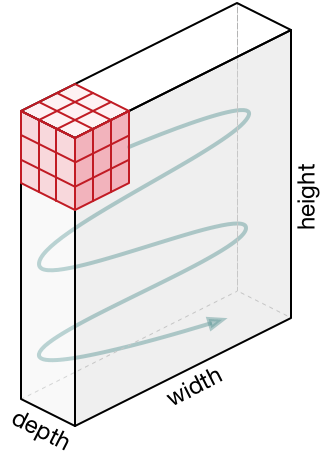
\includegraphics[scale=0.5]{chap2/c2_figs/13.png}
\end{center}
\caption{Phép tính convolution trên ảnh màu với k=3.}
\label{fig:padding,stride}
\end{figure}
\FloatBarrier

Ta định nghĩa kernel có cùng độ sâu (depth) với biểu diễn ảnh, rồi sau đó thực hiện di chuyển khối kernel tương tự như khi thực hiện trên ảnh xám.

\FloatBarrier
\begin{figure}[htp]
\begin{center}
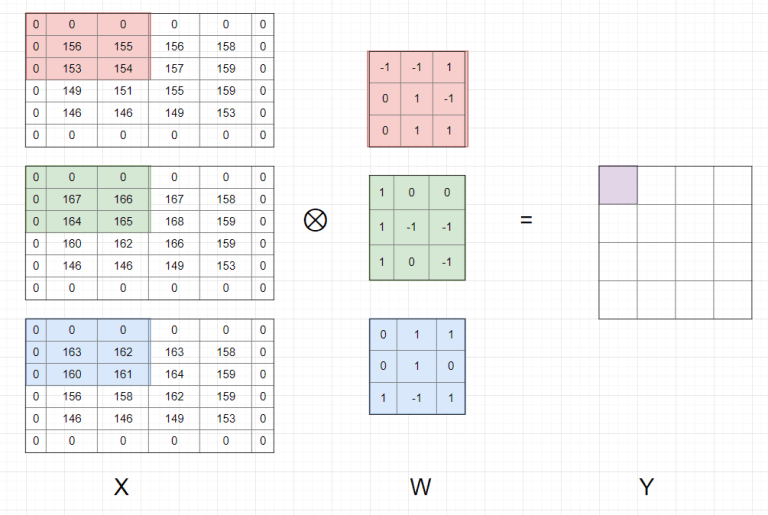
\includegraphics[scale=1]{chap2/c2_figs/14.png}
\end{center}
\caption{Tensor $X$ và $W$ 3 chiều được viết dưới dạng 3 matrix.}
\label{fig:padding,stride}
\end{figure}
\FloatBarrier

Khi biểu diễn ma trận ta cần 2 chỉ số hàng và cột: $i$ và $j$, thì khi biểu diễn ở dạng tensor 3 chiều cần thêm chỉ số độ sâu $k$. Nên chỉ số mỗi phần tử trong tensor là $x_{ijk}$.
$$y_{11} = b + (x_{111}*w_{111} +  x_{121}*w_{121} + x_{131}*w_{131} +  x_{211}*w_{211} +  x_{221}*w_{221} +  x_{231}*w_{231} +  x_{311}*w_{311} + $$ $$ x_{321}*w_{321} +  x_{331}*w_{331}) + (x_{112}*w_{112} +  x_{122}*w_{122} + x_{132}*w_{132} +  x_{212}*w_{212} +  x_{222}*w_{222} + $$ $$x_{232}*w_{232} +  x_{312}*w_{312} +  x_{322}*w_{322} +  x_{332}*w_{332}) +  (x_{113}*w_{113} +  x_{123}*w_{123} + x_{133}*w_{133} +  x_{213}*w_{213} + $$ $$ x_{223}*w_{223} +  x_{233}*w_{233} +  x_{313}*w_{313} +  x_{323}*w_{323} +  x_{333}*w_{333}) = -25$$

\FloatBarrier
\begin{figure}[htp]
\begin{center}
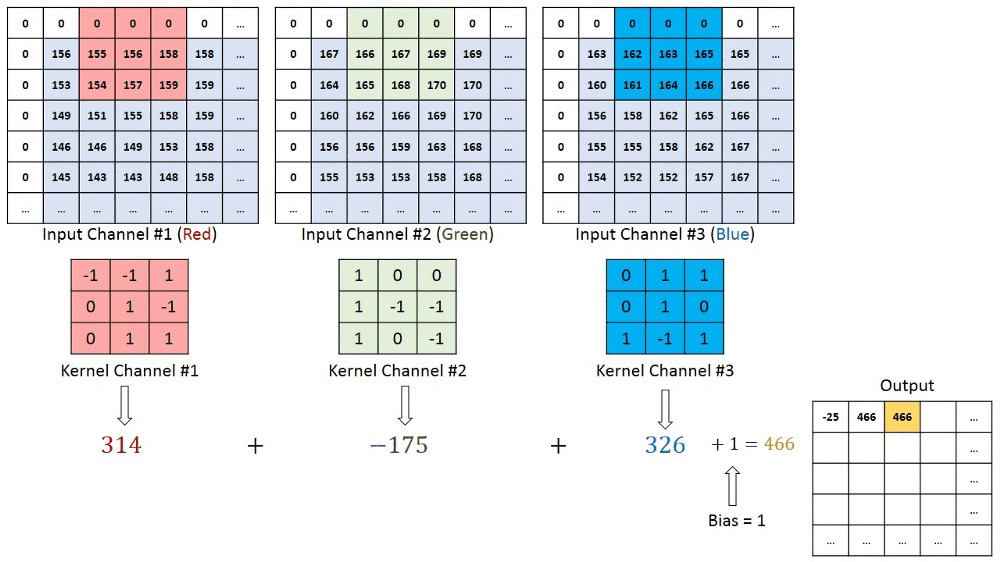
\includegraphics[scale=0.456]{chap2/c2_figs/8.jpg}
\end{center}
\caption{Thực hiện phép tính convolution trên ảnh màu}
\label{fig:padding,stride}
\end{figure}
\FloatBarrier

Nhận xét:
\begin{itemize}
\item Output Y của phép tính convolution trên ảnh màu là 1 matrix.
\item Có 1 hệ số bias được cộng vào sau bước tính tổng các phần tử của phép tính element-wise.
\end{itemize}

Với mỗi kernel khác nhau ta sẽ học được những đặc trưng khác nhau của ảnh, nên trong mỗi convolutional layer ta sẽ dùng nhiều kernel để học được nhiều thuộc tính của ảnh. Vì mỗi kernel cho ra output là 1 matrix nên k kernel sẽ cho ra k output matrix. Ta kết hợp k output matrix này lại thành 1 tensor 3 chiều có chiều sâu k.

\FloatBarrier
\begin{figure}[htp]
\begin{center}
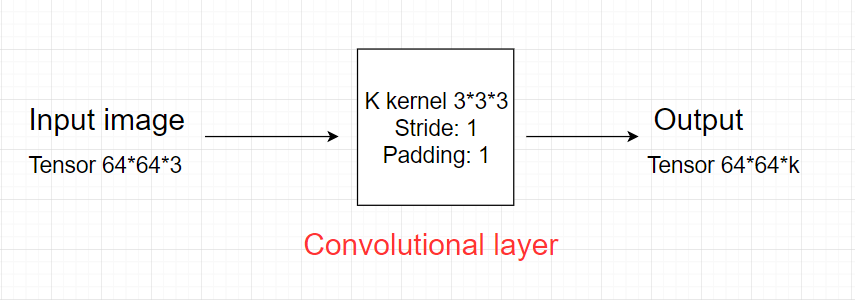
\includegraphics[scale=0.8]{chap2/c2_figs/15.png}
\end{center}
\caption{Convolutional layer đầu tiên}
\label{fig:conv-firstlayer}
\end{figure}
\FloatBarrier

Output của convolutional layer đầu tiên sẽ thành input của convolutional layer tiếp theo.

Convolutional layer tổng quát
Giả sử input của 1 convolutional layer tổng quát là tensor kích thước $H * W * D$.

Kernel có kích thước $F * F * D$ (kernel luôn có depth bằng depth của input và $F$ là số lẻ), stride: $S$, padding: $P$.

Convolutional layer áp dụng $K$ kernel.
=> Output của layer là tensor 3 chiều có kích thước: $ (\frac{H-F+2P}{S} + 1) * (\frac{W-F+2P}{S} + 1) * K$

\FloatBarrier
\begin{figure}[htp]
\begin{center}
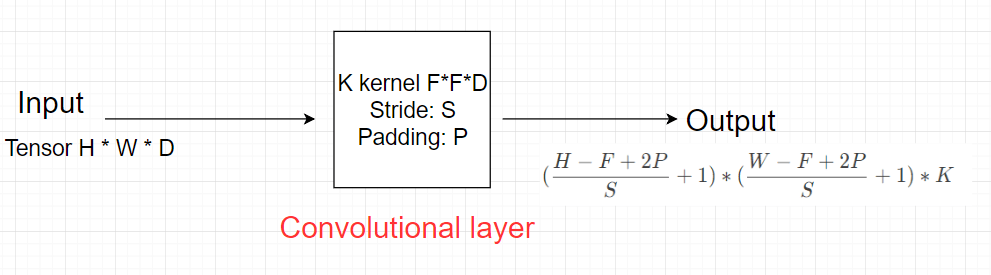
\includegraphics[scale=0.8]{chap2/c2_figs/16.png}
\end{center}
\caption{Convolutional layer tổng quát}
\label{fig:conv-tongquat}
\end{figure}
\FloatBarrier

Lưu ý:
\begin{itemize}
\item Output của convolutional layer sẽ qua hàm activation function trước khi trở thành input của convolutional layer tiếp theo.
\item Tổng số parameter của layer: Mỗi kernel có kích thước $F*F*D$ và có 1 hệ số bias, nên tổng parameter của 1 kernel là $F*F*D + 1$. Mà convolutional layer áp dụng $K$ kernel => Tổng số parameter trong layer này là $K * (F*F*D + 1)$.
\end{itemize}
Mạng Convolution Neural Network, ngoài các lớp Convolution ra còn có các lớp Pooling, Dropout, Dense, và Backnomalization,... để làm cho chúng trở nên "dễ học" hơn.


\subsection{Pooling layer}
\label{ss:Pooling}
Pooling layer thường được dùng giữa các convolutional layer, để giảm kích thước dữ liệu nhưng vẫn giữ được các thuộc tính quan trọng. Kích thước dữ liệu giảm giúp giảm việc tính toán trong model.

Gọi pooling size kích thước $K*K$. Input của pooling layer có kích thước $H*W*D$, ta tách ra làm $D$ ma trận kích thước $H*W$. Với mỗi ma trận, trên vùng kích thước $K*K$ trên ma trận ta tìm maximum hoặc average của dữ liệu rồi viết vào ma trận kết quả. Quy tắc về stride và padding áp dụng như phép tính convolution trên ảnh.

\FloatBarrier
\begin{figure}[htp]
\begin{center}
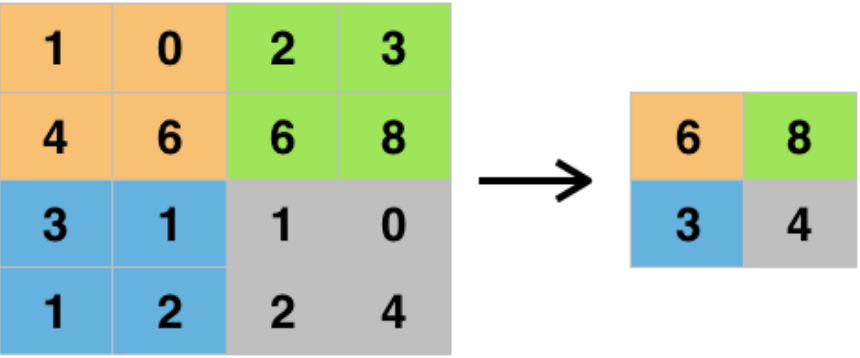
\includegraphics[scale=0.3]{chap2/c2_figs/9.jpg}
\end{center}
\caption{Phép Pooling với $stride=2, padding=0$}
\label{fig:pooling}
\end{figure}
\FloatBarrier

Nhưng hầu hết khi dùng pooling layer thì sẽ dùng $size=(2,2)$, $stride=2$, $padding=0$. Khi đó output width và height của dữ liệu giảm đi một nửa, depth thì được giữ nguyên.

\FloatBarrier
\begin{figure}[htp]
\begin{center}
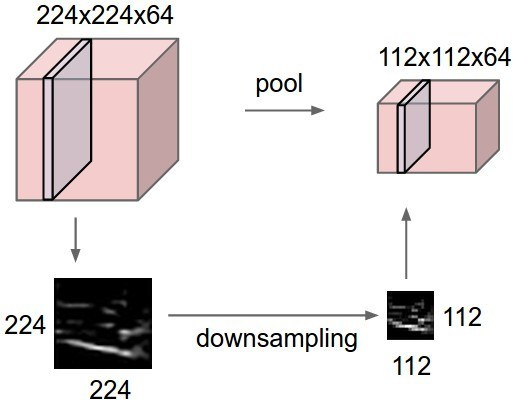
\includegraphics[scale=0.5]{chap2/c2_figs/pooling.jpeg}
\end{center}
\caption{Kết quả sau khi qua pooling layer $2*2$.}
\label{fig:pooling}
\end{figure}
\FloatBarrier
\centerline{http://cs231n.github.io/convolutional-networks/}

Có 2 loại pooling layer phổ biến là: max pooling và average pooling.
\FloatBarrier
\begin{figure}[htp]
\begin{center}
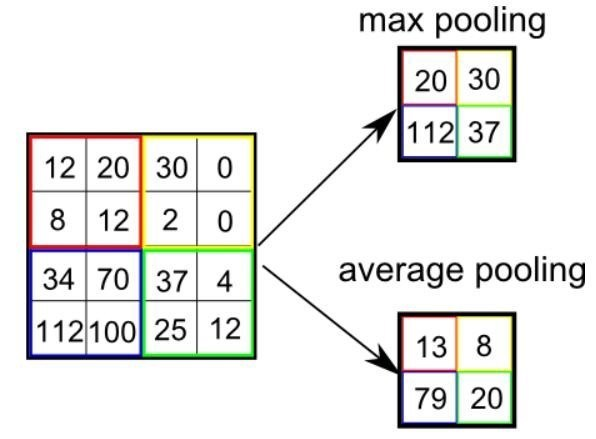
\includegraphics[scale=0.5]{chap2/c2_figs/10.jpg}
\end{center}
\caption{Max pooling và average pooling}
\label{fig:pooling}
\end{figure}
\FloatBarrier
Ngoài ra còn có thể dùng convolutional layer với stride > 1 để giảm kích thước dữ liệu thay cho pooling layer.

\subsection{Fully connected layer (Dense layer)}
\label{ss:dense}
Sau khi ảnh được truyền qua nhiều convolutional layer và pooling layer thì model đã học được tương đối các đặc điểm của ảnh (ví dụ mắt, mũi, khung mặt,…) thì tensor của output của layer cuối cùng, kích thước $H*W*D$, sẽ được chuyển về 1 vector kích thước $(H*W*D)$.

\FloatBarrier
\begin{figure}[htp]
\begin{center}
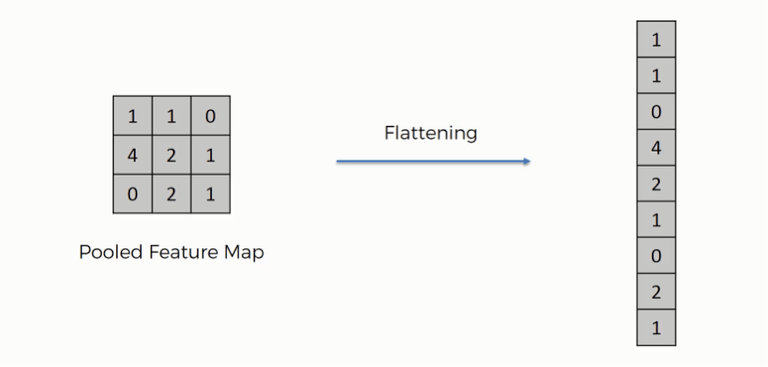
\includegraphics[scale=1]{chap2/c2_figs/17.png}
\end{center}
\caption{Phép Flatten biến tensor về 1 vector}
\label{fig:flatten}
\end{figure}
\FloatBarrier
Sau đó, mỗi điểm của vector sẽ được liên kết với toàn bộ output của mode giống như 1 lớp của mạng Neural Network truyền thống.Và cuối cùng của mạng sẽ có nhiệm vụ phân loại theo như yêu cầu của từng bài toán. Thường sẽ sử dụng hàm softmax để tính đầu ra cho lớp này.




\subsection{Kết luận}
Tổng hợp lại, một mô hình mạng CNN sẽ có cấu trúc chung gần giống như hình \ref{fig:tonghopCNN}

\FloatBarrier
\begin{figure}[htp]
\begin{center}
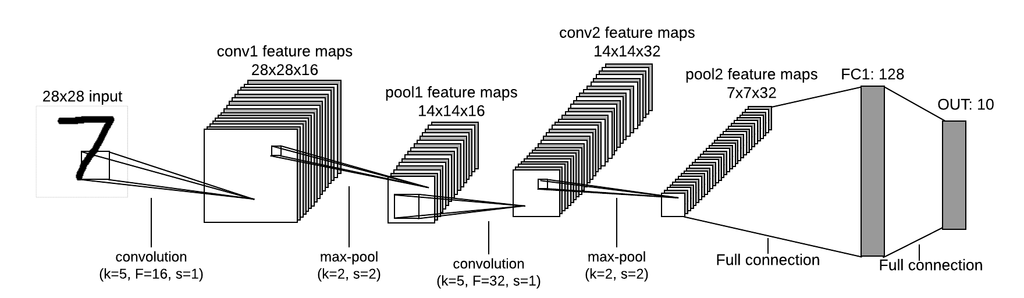
\includegraphics[scale=1]{chap2/c2_figs/18.png}
\end{center}
\caption{Ví dụ mô hình 1 môn hình convolutional neural network}
\label{fig:flatten}
\end{figure}
\FloatBarrier
\centerline{Input image -> Convolutional layer (Conv) + Pooling layer (Pool) -> Fully connected layer (FC) -> Output}
\centerline{Nguồn: https://www.easy-tensorflow.com/tf-tutorials/convolutional-neural-nets-cnns}